%%%%%%%%%%%%%%%%%%%%%%%%%%%%%%%%%%%%%%%%%%%%%%%%%%%%%%%%%%%%%%%
%
% Welcome to Overleaf --- just edit your LaTeX on the left,
% and we'll compile it for you on the right. If you open the
% 'Share' menu, you can invite other users to edit at the same
% time. See www.overleaf.com/learn for more info. Enjoy!
%
%%%%%%%%%%%%%%%%%%%%%%%%%%%%%%%%%%%%%%%%%%%%%%%%%%%%%%%%%%%%%%%
\documentclass{exam}
\usepackage{graphicx}
\usepackage{hyperref}
\usepackage{mathtools}
\begin{document}
{\LARGE\bf CSM2024: Homework 2 (85 points)}
\vspace{10mm}

\begin{questions}

\question (25 points)
\textbf{Ligand binding with depletion}

\begin{parts}
\part[10] Derive an expression for the fractional occupancy of a receptor R as a function of the total ligand and receptor concentrations, $L_{\mathrm{tot}}$ and $R_{\mathrm{tot}}$ respectively, and the binding dissociation constant $K_d$ \emph{without} assuming that ligand is in excess.
\part[5] Use this expression to make a plot of the fractional error in the binding probability from assuming ligand is in excess as a function of $L_{\mathrm{tot}}$.   Take $R_{\mathrm{tot}}=K_d=$ 50 nM. Interpret your result.
\part[10]
Fit the binding curves measured by \href{https://docs.google.com/spreadsheets/d/1ksNf_LojQfcdh_nQZClAYJAUvmLq8ssobo4LGYD_3wA/edit#gid=806736002}{Maeda et al.\ (2000)}
for binding of $\sigma^{70}$ to RNA polymerase assuming the $\sigma^{70}$ concentration is 0.4 nM using the expression you derived in part (a). Also fit the same data assuming that $L$ is in excess. Plot the fits and report the values of $K_d$ you obtain in each case. Note that the receptor in this case is $\sigma^{70}$ and the ligand concentrations are given in nM. What are your conclusions?
\end{parts}


\question (30 points)
\textbf{Network Motif Analysis}
\begin{parts}
\part[15]
Write a program to detect all 1, 2, and 3-mode motifs in a directed graph network. The input is a list of pairs of numbers indicating the source and target for each regulatory interaction. Apply your program to the E. coli network graph given  \href{https://www.weizmann.ac.il/mcb/UriAlon/sites/mcb.UriAlon/files/uploads/Network_motifs_in_coli/colinet-1.1.zip}{here}. Be sure to avoid overcounting subgraphs that occurs when a simple subgraph appears in a more complex one. In addition to your code provide a succinct description of the logic you used to find subgraphs and to avoid overcounting.
\part[15]
Write a program to generate ER networks with a given number of nodes and edges and use it to perform an analysis of your results in part (a) to determine which subgraphs are motifs or anti-motifs. Justify your choice of criteria for selecting these.
\end{parts}

\question (10 points)
\textbf{Linearized Positive Autoregulation}
Determine the response time for a linear model of positive autoregulation given by
$$ \frac{dX}{dt} = \beta + \beta_1 X - \alpha X$$
What assumptions do you need to make about the parameters?

\question (20 points)
\textbf{Shaping the Pulse}
In this problem we consider an I1-FFL as shown in the figure where gene X is initially not expressed but is turned on by simple gene regulation at time $t=0$. Assume that genes X, Y, and Z are expressed at rates $\beta_X$, $\beta_Y$, and $\beta_Z$ respectively when their promoters are in the ON state and 0 otherwise. Let the thresholds for each regulatory arrow shown be $K_{XY}$, $K_{XZ}$, and $K_{YZ}$.
Assume that the degradation rate for all three proteins has the same value $\alpha$.
Finally, assume that the signals regulating X and Y are present throughout.
\begin{figure}[h]
\begin{center}
    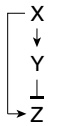
\includegraphics[scale=0.5]{iFFL-type1.jpg}
\end{center}
\caption{I1-FFL.}
\end{figure}
\begin{parts}
\part[5]
Make a figure showing how the pulse shape (width and height) depends on the model parameters.
\part[10]
Derive expressions for the pulse width and height as a function of the model parameters.
\part[5]
Design thresholds such that genes $Z_1$ and $Z_2$ regulated by the same circuit turn on and off in the same order and make a figure illustrating why this design works.
\end{parts}
\end{questions}
\end{document}
